\documentclass[12pt]{article}

\usepackage[utf8]{inputenc}
\usepackage[russian]{babel}
\usepackage{amsmath}
\usepackage{setspace}

\usepackage{caption}
\usepackage{subcaption}
\usepackage{float}
\usepackage{graphicx}
\graphicspath{ {./images/} }

\usepackage{geometry}
 \geometry{
 a4paper,
 left=20mm,
 right=20mm,
 top=20mm,
 bot=20mm,
 }

\begin{document}

\begin{titlepage}
\begin{center}
    {\small НАЦИОНАЛЬНЫЙ ИССЛЕДОВАТЕЛЬСКИЙ УНИВЕРСИТЕТ ИТМО} \\
    {\small Факультет систем управления и робототехники} \\
    \vspace*{10\baselineskip}
    {\LARGEЭлектроника и схемотехника} \\
    \ \\
    \begin{spacing}{1.5}
    {\large Лабораторная работа №3 \\
    Исследование исследование характеристик полевого транзистора} \\
    \end{spacing} \\
    \ \\
    Вариант 2 \\
    \vspace*{10\baselineskip}
    \hfill {Выполнили студенты:} \\
    \hfill {Кирбаба Д.Д. R3338} \\
    \hfill {Курчавый В.В. R3338} \\
    \ \\
    \hfill {Преподаватель:} \\
    \hfill {Николаев Н.А.} \\
    \mbox{}
    \vfill {г. Санкт-Петербург\\2023}
\end{center}
\end{titlepage}

\section*{Цель работы}
\begin{itemize}
  \item Получение передаточной характеристики, зависимости сопротивления канала полевого транзистора от напряжения затвор-исток и семейства выходных характеристик полевого транзистора;
  \item Расчёт схемы автоматического смещения полевого транзистора.
\end{itemize}

\section*{Ход работы}
Вариант 2.\\
Технические характеристики транзистора АО6608\_N: 
\begin{itemize}
    \item МОП полевой транзистор c индуцированным N-каналом;
    \item $I_{D_{max}} = 3.4 \ A$;
    \item $V_{SD_{max}} = 30 \ V$;
    \item $V_{GS_{th}} = 0.5 ... 1.5 \ V$;
    \item $P_D = 1.25 \ W$.
\end{itemize}

\begin{figure}[H]
    \centering
    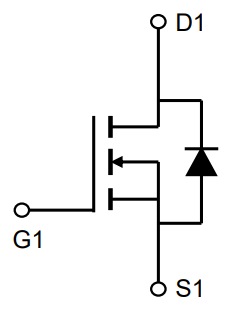
\includegraphics[width=0.2\textwidth]{transistor_scheme.png}
    \caption{Обозначение транзистора AO6608\_N.}
    \label{fig:transistor_scheme}
\end{figure}

\subsubsection*{Получение передаточной характеристики полевого транзистора в схеме с общим истоком}
\begin{figure}[H]
    \centering
    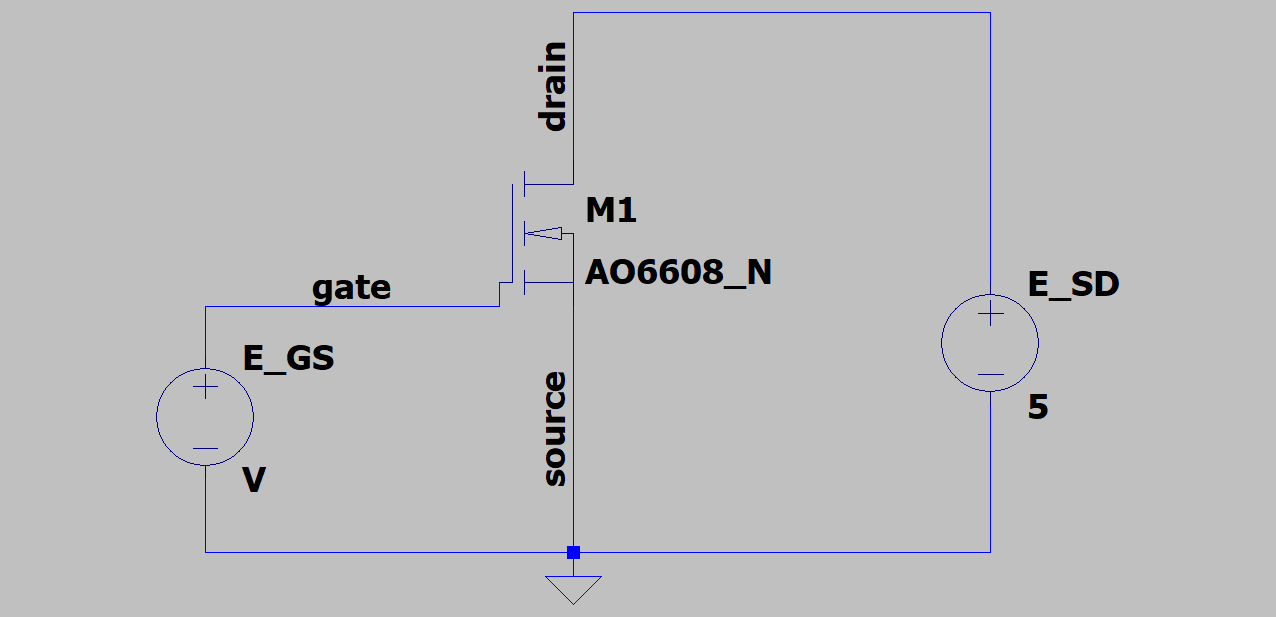
\includegraphics[width=0.7\textwidth]{1_scheme.png}
    \caption{Схема моделирования работы полевого транзистора.}
    \label{fig:1_scheme}
\end{figure}

Приведем график входной характеристики транзистора при $V_{SD} = 5 \ V$ и $V_{GS} \in [0, \ 1.5] \ V.$
\begin{figure}[H]
    \centering
    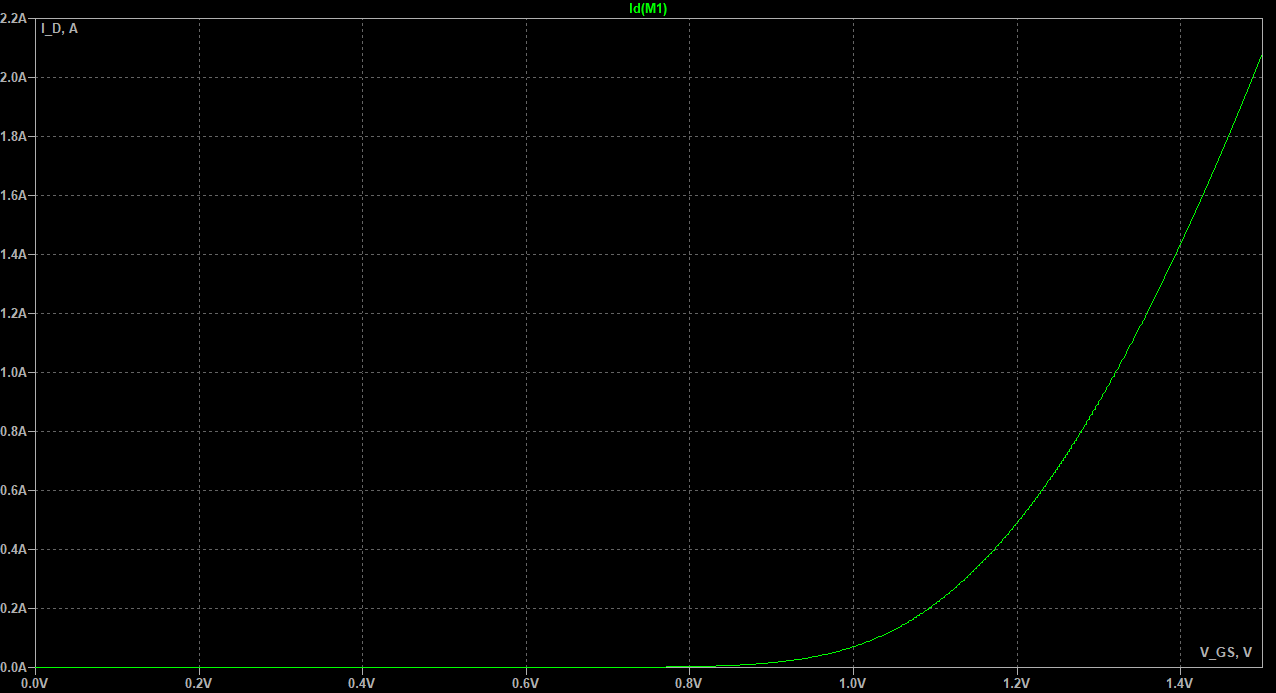
\includegraphics[width=\textwidth]{1_input_char.png}
    \caption{Входная характеристика.}
    \label{fig:1_input_char}
\end{figure}
Пороговое значение $V_{th} = 0.8 \ V$.\\
Выберем две точки на данной характеристике:
\[
    V_{GS_1} = 1.2225 \ V, \ I_{D_1} = 0.5697 \ A, \ V_{GS_2} = 1.4818 \ V, \ I_{D_2} = 1.9528 \ A.
\]
Вычислим крутизну передаточной характеристики полевого транзистора:
\[
    S = \frac{I_{D_2} - I_{D_1}}{V_{GS_2} - V_{GS_1}} = \frac{1.3831}{0.2593} = 5.334
\]
Определим значение удельной кривизны при $V_{GS_{mean}} = \frac{V_{GS_2} + V_{GS_1}}{2} = 1.35215 \ V$:
\[
    b = \frac{S}{V_{GS_{mean}} - V_{th}} = \frac{5.334}{1.35215 - 0.8} = 9.66
\]

\subsubsection*{Получение семейства выходных характеристик полевого транзистора в схеме с общим истоком}
$V_{SD} \in [0, \ 30] \ V, \ V_{GS} \in \{0.8, \ 0.975, \ 1.15, \ 1.325, \ 1.5\} \ V.$
\begin{figure}[H]
    \centering
    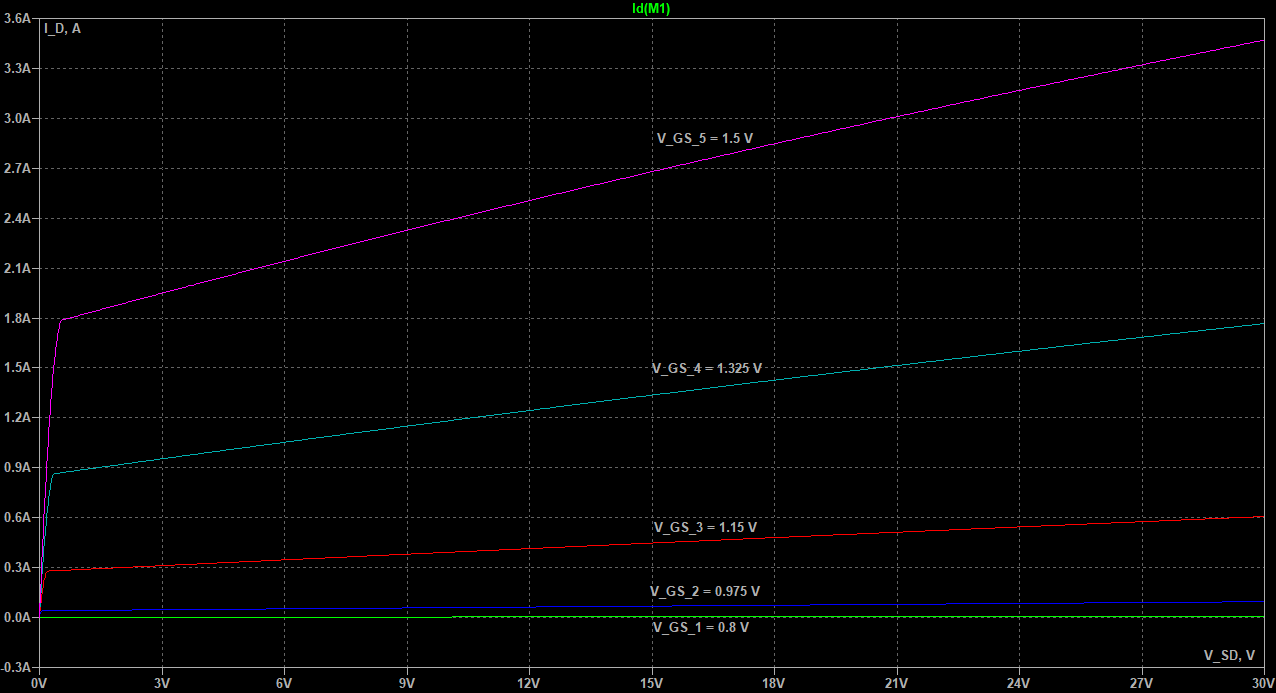
\includegraphics[width=\textwidth]{2_output_char.png}
    \caption{Семейство выходных характеристик полевого транзистора.}
    \label{fig:2_output_char}
\end{figure}
Для каждой полученной выходной характеристики получим значение тока стока, соответствующее $V_{SD} = 5 \ V$:
\[
    I_{D_1} = 0.002919 \ A, \ I_{D_2} = 0.05050 \ A, \ I_{D_3} = 0.3352 \ A, \ I_{D_4} = 1.02041 \ A, \ I_{D_5} = 2.07794 A.
\]
Вычислим соответствующие им значения крутизны $S = \sqrt{2 b I_D}$:
\[
    S_1 = 0.2375, \ S_2 = 0.9878, \ S_3 = 2.5448, \ S_4 = 4.44, \ S_5 = 6.336.
\]
Для ПТИЗ с индуцированным каналом верно, что при напряжении на затворе меньше порогового значения $V_{th} = 0.8 \ V$ ток стока транзистора равен нулю, а его появление происходит только при большем напряжении на затворе, и в дальнейшем, при увеличения напряжения на затворе происходит увеличение тока стока. \\
Так как мы получили выходные характеристики при различных значениях напряжения на затворе и зафиксировали напряжение на истоке-стоке, то величина крутизны будет различно и характеризовать усилительные свойства. \\
\ \\
Значение крутизны, вычисленное ранее $S = 5.334$. \\
Это значение является средним усилением транзистора между выбранными точками $V_{GS_1}$ и $V_{GS_2}$. \\
Логично, что крутизна будет нарастать с увеличением протекающего через канал тока.

\subsubsection*{Расчет усилительного каскада на полевом транзисторе}

Исходные данные: $R_{load} = 200 \ Ohm, \ V_{load_{max}} = 5 V$.

\begin{figure}[H]
    \centering
    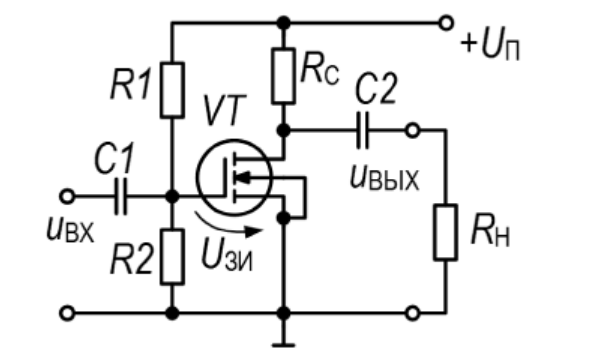
\includegraphics[width=0.4\textwidth]{3_book_scheme.png}
    \caption{Схема усилительного каскада на полевом транзисторе с изолированным затвором.}
    \label{fig:3_book_scheme}
\end{figure}

Отобразим линию максимальной мощности на семействе ВАХ:
\begin{figure}[H]
    \centering
    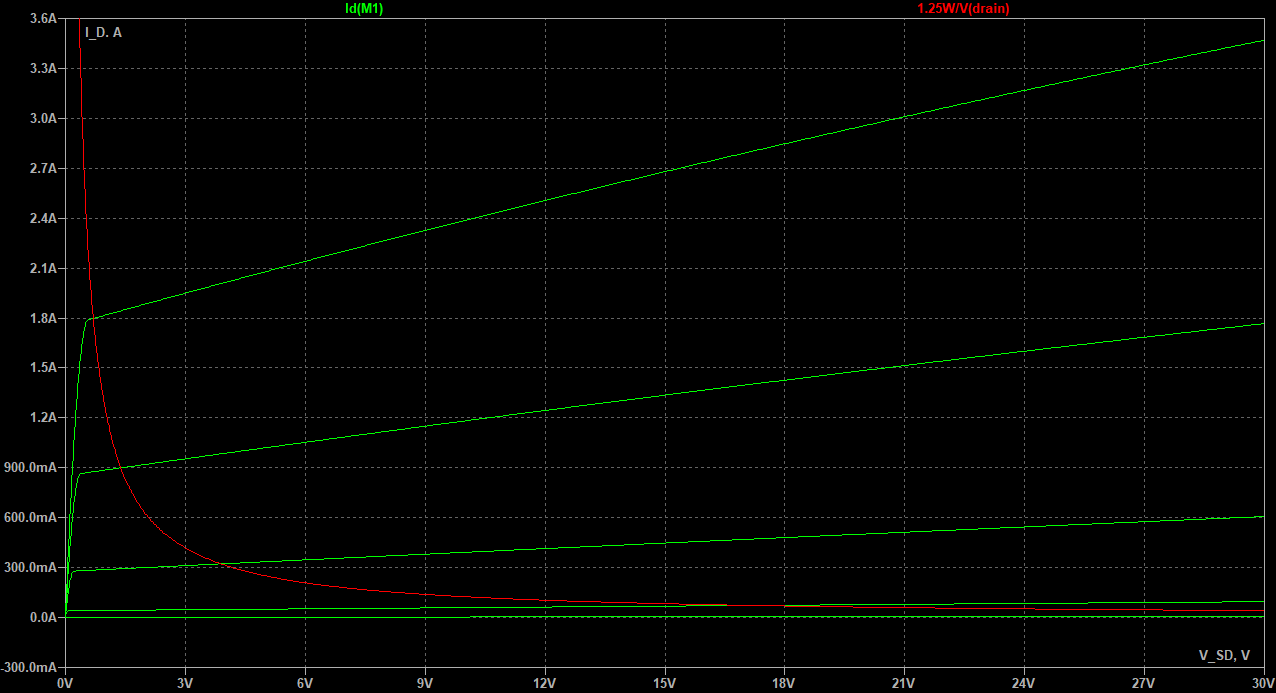
\includegraphics[width=\textwidth]{2_output_char_w_load_line.png}
    \caption{Семейство выходных характеристик полевого транзистора с нагрузочной линией.}
    \label{fig:2_output_char_w_load_line}
\end{figure}

Изменим токи на истоке-затворе и масштаб:
\begin{figure}[H]
    \centering
    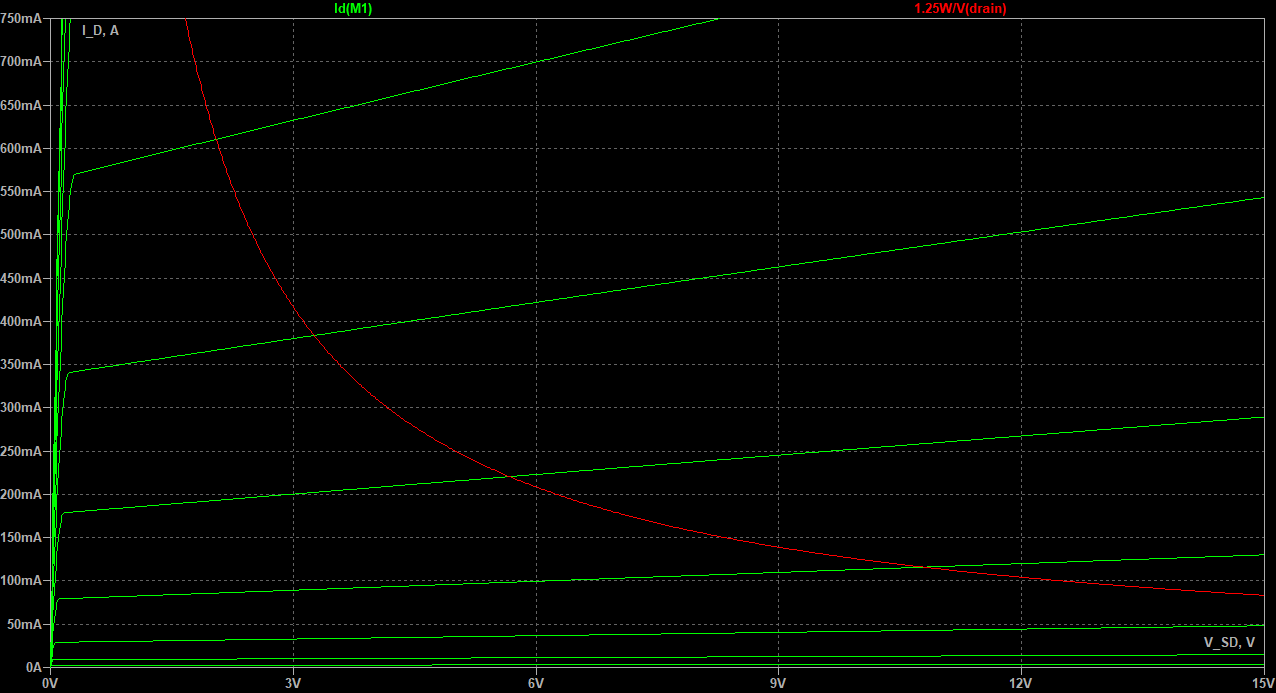
\includegraphics[width=\textwidth]{2_output_with_max_power_line_small.png}
    \caption{Семейство выходных характеристик полевого транзистора с нагрузочной линией.}
    \label{fig:2_output_with_max_power_line_small}
\end{figure}

Для нормальной работы усилительного каскада необходимо установить определенные токи и напряжения во входной и выходной цепях транзистора при отсутствии входного сигнала. Такой режим работы называют \emph{режимом покоя}. \\

Точка, координаты которой на ВАХ транзистора определяют напряжения и токи в его электродах, называется \emph{рабочей}. При отсутствии входного сигнала эта точка называется \emph{исходной рабочй точкой} (И.Р.Т.). Исходная рабочая точка определяет режим работы транзистора по постоянному току. \\

Выберем рабочую точку транзистора и нанесем нагрузочную линию:
\begin{figure}[H]
    \centering
    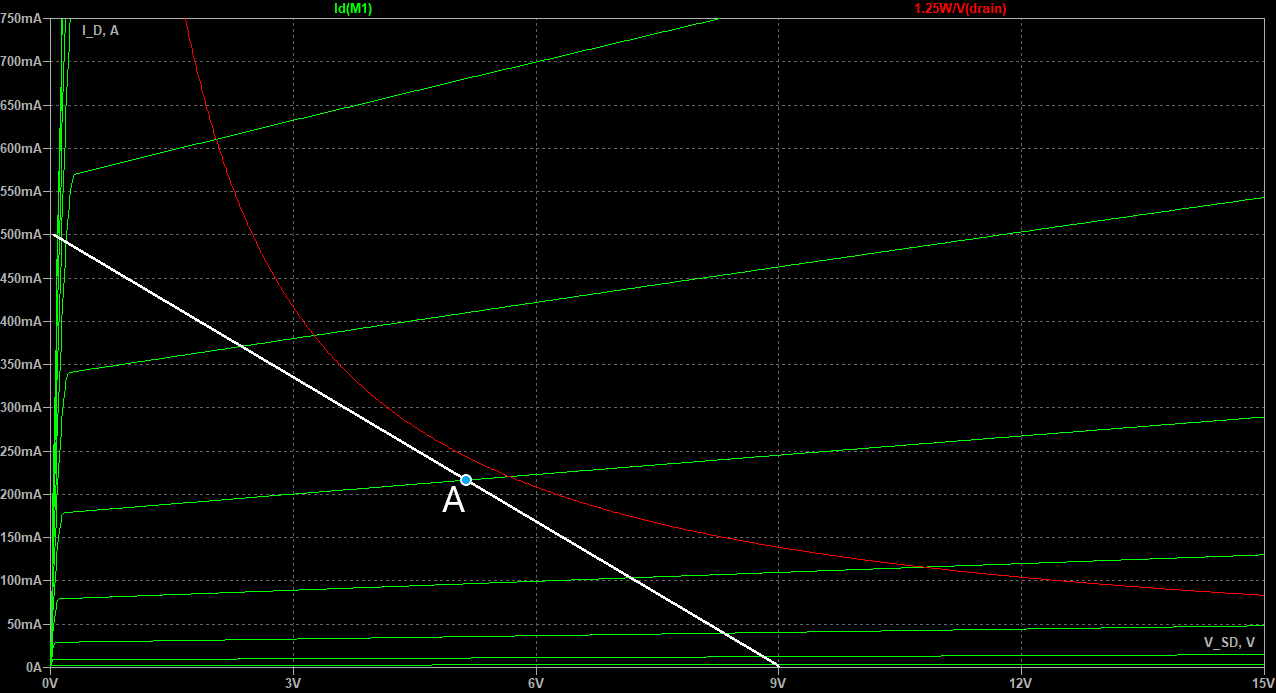
\includegraphics[width=\textwidth]{2_output_with_max_power_line_small_and_load_line_and_work_dot.png}
    \caption{Рабочая точка и нагрузочная линия.}
    \label{fig:2_output_with_max_power_line_small_and_load_line_and_work_dot}
\end{figure}

Характеристики рабочей точки:
\[
    V_{GS_0} = 1.1 \ V, \ \ V_{SD_0} = 5.07825 \ V, \ \ I_{D_0} = 0.21606225 \ A.
\]
\[
    V_{supp} = 9 \ V, \ \ I_{D_{max}} = 0.5 \ A.
\]

Рассчитаем выходную мощность и максимальный ток в нагрузке:
\[
    P_{out} = \frac{V_{load_{max}}^2}{2R_{load}} = 0.0625 \ W, \ \ I_{load_{max}} = \frac{V_{load_{max}}}{R_{load}} = 0.025 \ A.
\]

В каскаде, изображенном на рисунке 5, транзистор $VT$ совместно с резистором $R_C$ образуют управляемый делитель напряжения. С помощью остальных резисторов реализуют цепи, обеспечивающие начальный режим работы транзистора. Разделительные конденсаторы $C_1$ и $C_2$ служат соответственно для предотвращения проникновения постоянной составляющей сигнала на затвор транзистора и на выход усилительного каскада. Их значения выберем равными $1 \ mcF$.

Сопротивление $R_C = \frac{V_{supp}}{I_{D_{max}}} = 18 \ Ohm$. \\
\ \\
Проверим выполнение условий: 
\[
    V_{SD_{max}} = 30 \ V > V_{supp} = 9 \ V;
\]
\[
    I_{D_{max}} = 3.4 \ A > I_{D_{max}} = 0.5 \ A;
\]
\[
    P_{D_{max}} = 1.25 \ W > V_{SD_0} I_{D_0} = 1.097 \ W.
\]

Задаваясь значением $R_1 || R_2 = 4.95 \ MOhm$ находим:
\[
    R_1 = \frac{V_{supp}}{V_{GS_0}} 4.95 = 40.5 \ MOhm;
\]
\[
    R_2 = \frac{V_{GS_0}}{V_{supp} - V_{GS_0}} R_1 = 5.639 \ MOhm.
\]

\begin{figure}[H]
    \centering
    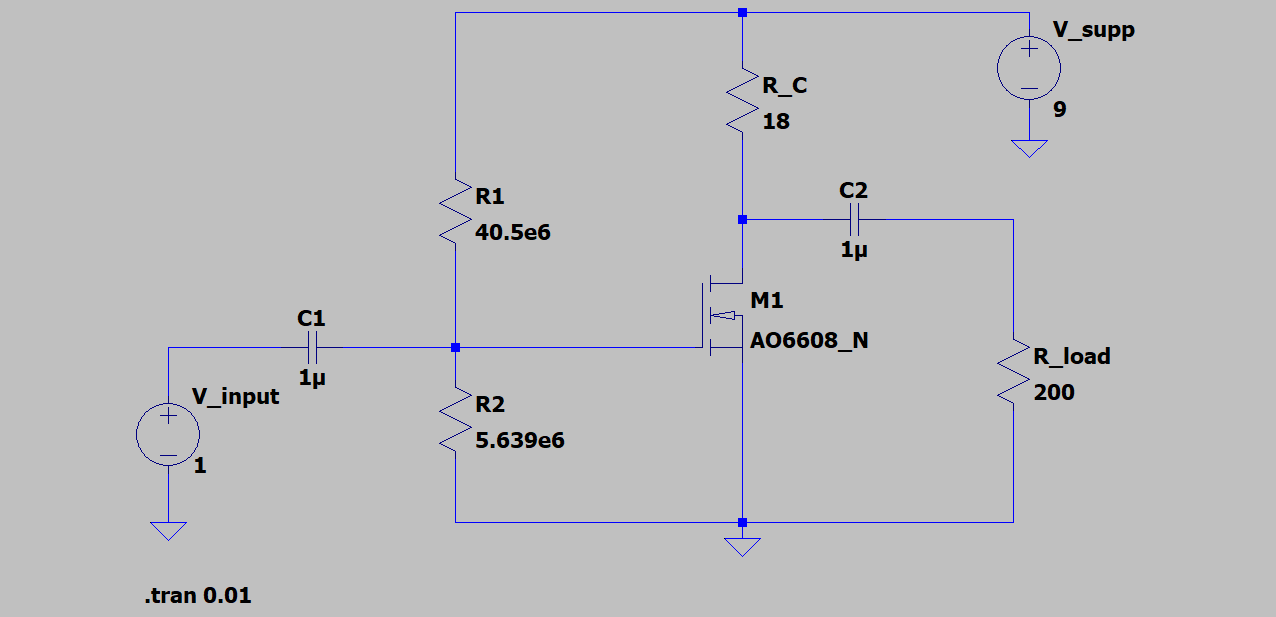
\includegraphics[width=\textwidth]{3_scheme.png}
    \caption{Схема моделирования усилительного каскада.}
    \label{fig:3_scheme}
\end{figure}

Произведем моделирование работы схемы при постоянном входном сигнале $U_{input} = 1 \ V$:
\begin{figure}[H]
    \centering
    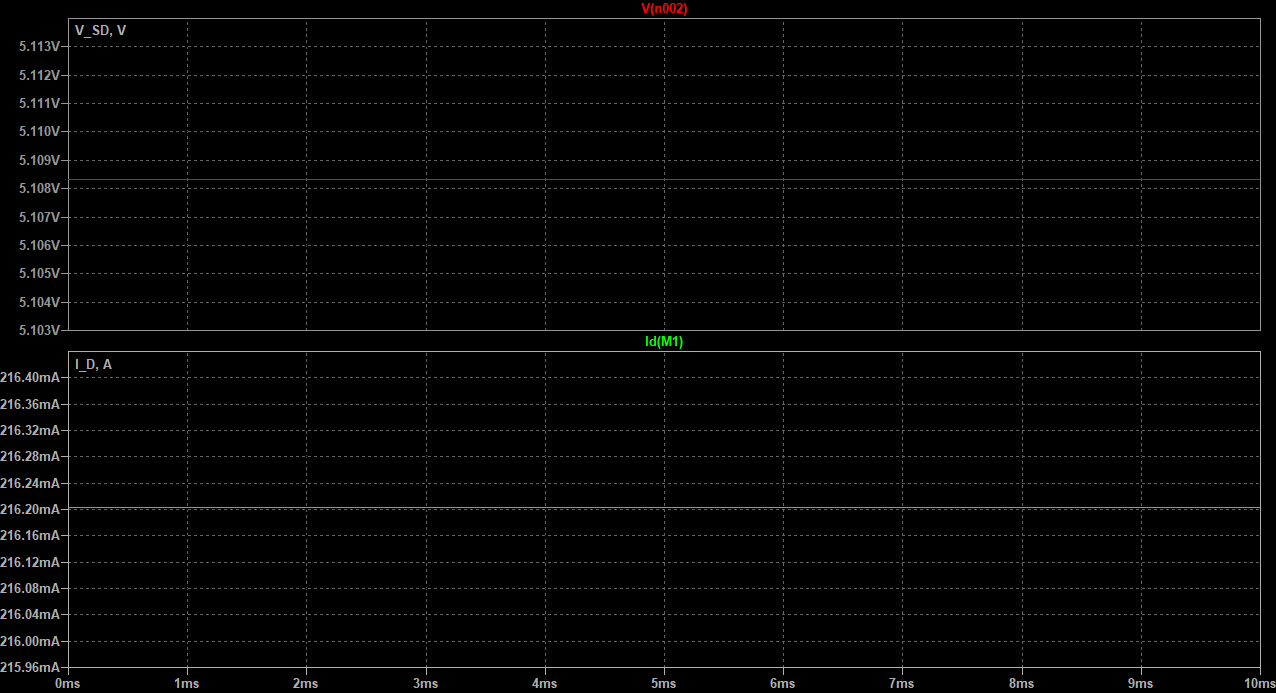
\includegraphics[width=\textwidth]{3_const_signal.png}
    \caption{Осциллограммы выходных тока и напряжения при постоянном сигнале.}
    \label{fig:3_const_signal}
\end{figure}

Выходные значения тока и напряжения близки к значениям заданной рабочей точки, значит расчет элементов усилительного каскада был проведен верно. \\
\ \\
Произведем моделирование работы схемы при гармоническом входном сигнале $U_{input} = 0.1 \sin{1000 t}$:
\begin{figure}[H]
    \centering
    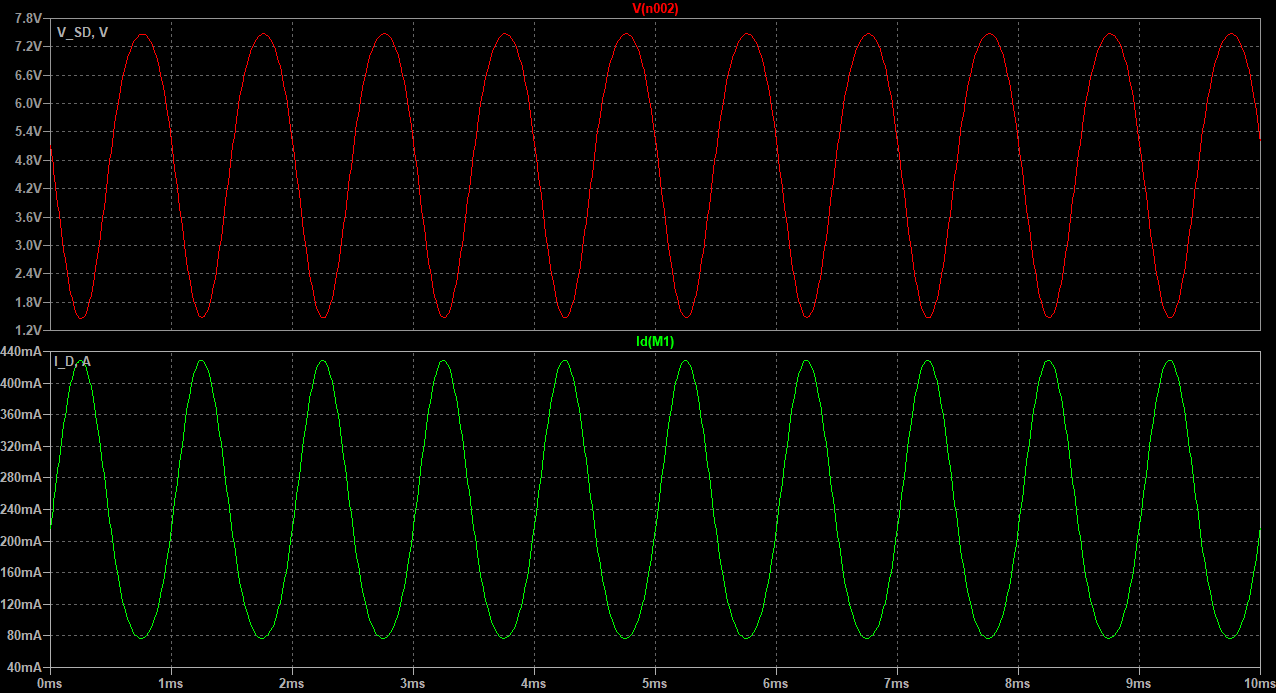
\includegraphics[width=\textwidth]{3_sin_signal.png}
    \caption{Осциллограммы выходных тока и напряжения при синусоидальном сигнале.}
    \label{fig:3_sin_signal}
\end{figure}

Данный усилительный каскад работает в режиме калсса \emph{A}, так как мы выбрали рабочую точку, находящуюся на линейном участке входной характеристики и амплитуда входного сигнала такова, что транзистор входит в насыщения. \\
\ \\
Теперь рассчитаем коэффициент усиления по напряжению как отношение амплитуды выходного напряжения к входному:
\begin{figure}[H]
    \centering
    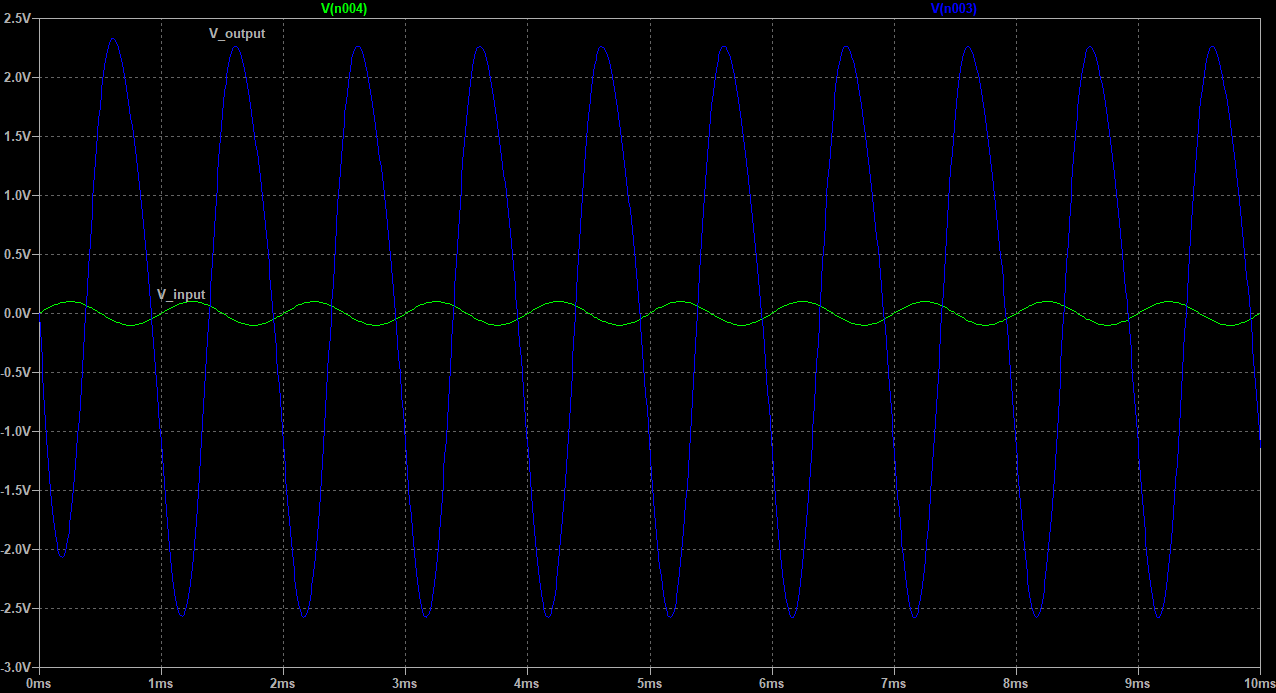
\includegraphics[width=\textwidth]{3_v_in_out.png}
    \caption{Осциллограммы входного и выходного напряжения при синусоидальном сигнале.}
    \label{fig:3_v_in_out}
\end{figure}
\[
    k_V = \frac{V_{out_{amp}}}{V_{in_{amp}}} = \frac{2.26543}{0.1} = 22.6543
\]

\section*{Выводы}
В данной лабораторной работе было проведено исследование свойств полевого транзистора с индуцированным n-каналом. МОП транзистор обогащенного типа в нормальном состоянии закрыт и проводит ток только тогда, когда приложено напряжение $V_{GS}$ выше порогового $V_{th} = 0.8 \ V$. Это было подтверждено моделированием и построением входной характеристики. \\ 
Во второй части работы была построена стоковая (выходная) характеристика транзистора. В целом, её вид аналогичен с выходной характеристикой из прошлой лабораторной работы, за исключением того, что при $V_{GS}<V_{th}$ характеристика будет сливаться с осью абсцисс. На данном семействе выходных характеристик выделяют 4 области: отсечки, насыщения, пробоя, омическая. Также в конце была вычислена крутизна транзистора - скорость изменения тока стока в зависимости от изменения напряжения затвор-исток при фиксированном значении  напряжения сток-исток.
\\
В заключительной части был проведен расчет усилительного каскада на полевом транзисторе. Была выбрана рабочая точка и она стабилизировалась с помощью схемы автоматического смещения с делителем напряжения. Из-за того, что рабочая точка была выбрана на линейном участке входной характеристики и амплитуда входного сигнала подобрана так, что транзистор входит в насыщения, то усилительный каскад работал в классе \emph{A}.

\end{document}